\chapter{Méthodologie}
\minitoc%

\warn{toute la rédaction de ce chapitre est une ébauche grossière, destinée à former le squelette du rapport. Le processus de rédaction est itératif sur toute la durée du stage. avancement du stage : 2 / 6 mois}


\section{Données Fonctionnelles : l'essentiel}
    \subsection{Cas indépendant : données fonctionnelles}

    \subsection{Cas non indépendant : séries temporelles de données fonctionnelles}
        
    Une large partie de la théorie des données fonctionnelles suppose que l'on observe des courbes $X_i : \Omega \rightarrow \mathcal C^0(I, \mathds R)$ \textbf{indépendantes} et identiquement distribuées. Cependant une partie non négligeable des données que l'on observe ont des dépendances avec les valeurs passées. Par exemple, il est raisonnable de penser que la consommation électrique d'un foyer au cours d'une année croît avec l'ajout successif de nouveau appareils électroniques. L'hypothèse d'indépendance entre les données n'est donc plus pertinente pour les données que l'on traite et il devient important de considérer des processus autorégressifs adaptés aux données fonctionnelles. 
Si dans le cadre des données de $\mathds R$ cette relation de \emph{dépendance linéaire} avec le passé pouvait s'écrire sous la forme suivante 
$X_n = \sum\limits_{k=1}^{n-1} \varphi_k \, X_k + \varepsilon_n$ où $\varphi_k \in \grandR$ 
et 
$\varepsilon_n \begin{cases} \in \operatorname{VA}(\grandR) \\ \indep \sigma\left( X_i \right)_{1\,: \, n-1}\end{cases}$, 
dans le cadre fonctionnel on capture la même idée en considérant 
$X_n = \sum\limits_{k=1}^{n-1} \phi_k \left( X_k \right) + \varepsilon_n$ où $\phi_k$ 
est un \emph{opérateur linéaire} de $\mathds L^2(I, \mathds R)$, 
le plus souvent intégral. 

\chk{
    Il s'agit d'une généralisation naturelle de la relation dans le cadre réel, puisqu'on peut démontrer que sur l'espace des nombres réels l'ensemble des fonctions linéaires $\phi : \grandR \rightarrow \grandR$ sont de la forme $x \mapsto ax$ avec $a \in \grandR$. La relation sur $\grandR$ que l'on a vue juste avant peut alors se ré-écrire de façon similaire à la version fonctionnelle.
    }

\section{Estimation de la régularité locale des trajectoires}

\subsection{Ce qu'on entend par régularité locale}

Longtemps, il était cru que les fonctions continues étaient dérivables presque partout. C'est notamment Weierstrass qui a démontré qu'il existe des fonctions continues partout mais dérivable nulle part. Poincaré notamment disait de tels objets qu'ils n'existaient que pour contredire le travail des pères. 
% @ todo : ⚠️ pertinence de l'intro 
\editorwarn{s'assurer de la pertinence : Holder => UC ce qui est quand même bien plus régulier que continu dans le cadre de la fonction de Weierstrass}
Cependant, des objets manipulés tous les jours comme le monde de la finance notamment traitent des processus qui sont fondamentalement irréguliers (au point de vue de l'analyse, où l'on traite souvent des fonctions au moins dérivables). Il est donc important de pouvoir quantifier la régularité d'une fonction de façon plus fine que le nombre de dérivées qu'elle possède. 

Nous allons repasser rapidement en revue les différents concepts de régularité pour mettre l'emphase dans ce que l'on considère comme régularité locale.

Afin de savoir à quel niveau de régularité nous souhaitons estimer, il est important de garder en tête un ordre de différents niveaux de régularité résumé par les relations suivantes :

$$\textsf{Lipschitz} \implies \textsf{Hölder} \implies \underbracket{\colorize{\textsf{Localement Hölder}}}_{\textsf{ce qui nous intéresse}} \implies \textsf{Uniformément continue} \implies \textsf{Continue}$$

\begin{itemize}
    \item Continuité :
    $$(\forall \varepsilon > 0) \, (\forall x) (\exists \delta_{\colorize x} > 0) (\forall y) \, |x-y| < \delta \implies |f(x) - f(y)| < \varepsilon$$
    \item Uniforme Continuité :
    $$(\forall \varepsilon > 0) \, (\exists \delta > 0) (\forall x,y ) \, |x-y| < \delta \implies |f(x) - f(y)| < \varepsilon$$
    \item Lipschitz :
    $$(\forall x,y) \quad |f(x) - f(y)| < L |x-y|$$
    \item Hölder :
    $$
    \begin{cases}
    (\forall x,y) \quad |f(x) - f(y)| < L_\alpha |x-y|^\alpha
    \\
    0 < \alpha \leq 1 
    \end{cases}
    $$
    \brain{
    une fonction lipschitz est une fonction Holderienne avec $\alpha = 1$
    }

    \item Localement Hölder :
    $$
    \forall x_0 \quad \begin{cases}
    (\forall x) \quad |f(x) - f(x_0)| < L_{\alpha(x_0)} |x-x_0|^{\alpha(x_0)}
    \\
    \quad 0 < {\alpha(x_0)} \leq 1 
    \end{cases}
    $$
\end{itemize}

\question{
    \smallskip\centering
    Pourquoi se concentrer sur des processus localement Hölder ?
}

La nature des phénomènes rencontrés dans la vie réelle est souvent complexe. Influencés par de nombreux phénomènes, certains d'entre eux sont, comme mentionnés précédemment, irréguliers. C'est notamment le cas des courbes de charge électriques, qui dépendent de multitudes de phénomènes physiques ou comportementaux, dont on peut attendre une certaine régularité, mais qui ne sont pas nécessairement uniformes tant sur leur niveau régularité que l'intervalle de temps sur lequel ils ont une influence. On pourrait par exemple attendre une différence de régularité de la production électrique en plein été (soleil et température stables \ldots) comparé au mois de mars (plus grande instabilité des conditions climatiques).

De plus, les fonctions Hölderiennes représentent une classe suffisamment large de fonctions. L'espace de fonctions sur lequel on travail est donc devrait être en pratique suffisamment grand pour inclure l'ensemble des processus qui nous intéressent.




\subsection{Estimation des paramètres régularité locale des trajectoire}




\subsection{Prélissage : lissage à ondelettes}

Afin de pouvoir estimer la régularité locale des trajectoires, nous allons lisser les trajectoires. En effet, celles-ci sont souvent bruitées, et il est nécessaire de lisser les trajectoires afin de pouvoir estimer la régularité locale de façon pertinente. De plus si on veut estimer la régularité en un point non observé, il devient alors nécessaire de lisser les trajectoires afin de pouvoir estimer la régularité en ce point. Cette étape de lissage est appelée prélissage de la courbe.

\question{
    \smallskip\centering
    Pourquoi parle-t-on de \textbf{pré}-lissage ? Le but de considérer la régularité n'était-il pas justement de l'utiliser dans le lissage des trajectoires ? Lisser avant même d'estimer la régularité n'est-il pas contre-productif ?
}

L'objectif de l'obtention des paramètres de régularité des trajectoires est de pouvoir effectuer un lissage de ces trajectoires qui préserve les irrégularités fondamentales du processus dont elles sont issues, tout en éliminant le bruit. Les paramètres de régularité sont donc dans un premier temps estimés en utilisant des trajectoires lissées puis utilisés pour effectuer un nouveau lissage à noyaux en utilisant une fenêtre de lissage appropriée qui dépend de ces paramètres. 
% @ todo : expression de h_𝛼(t)
\editorwarn{inclure l'expression de $h_\alpha(t)$}
% @ ————————————


\subsubsection{Une brève introduction aux ondelettes}


Les ondelettes proviennent du monde du traîtement du signal. Elles répondent à un problème de représentation des données à la fois dans le domaine temporel et dans le domaine fréquentiel. En effet, la transformée de Fourier nous donne accès aux fréquences présentes dans un signal mais ne nous permet pas de localiser à quel moment sont intervenues les fréquences spécifiques. Le théorème d'indétermination de Heisenberg stipule que l'on ne peut avoir une résolution parfaite à la fois dans le domaine fréquentiel et le domaine temporel, il y a un compromis qui doit être fait. La question devient alors :

\question{
    \smallskip\centering
    Comment représenter une fonction dans le domaine temporel et dans le domaine fréquentiel de façon optimale ? En d'autres termes, quelle résolution temporelle et quelle résolution fréquentielle choisir ?
}

Une première approche proposée en 
% @ todo : compléter date et auteur — STFT
\editorwarn{compléter date} par \editorwarn{compléter auteur}
% @ ————————————
est la transformée de Fourier à court terme (STFT). Celle-ci consiste à regarder la transformée de Fourier d'une fonction sur une fenêtre de taille fixe et à faire glisser cette fenêtre sur la fonction. On obtient ainsi la représentation fréquentielle de la fonction sur un intervalle de temps centré en un point que l'on peut faire varier. 

\bigskip

\begin{minipage}{0.32 \textwidth}
    \begin{figure}[H]
        \centering
        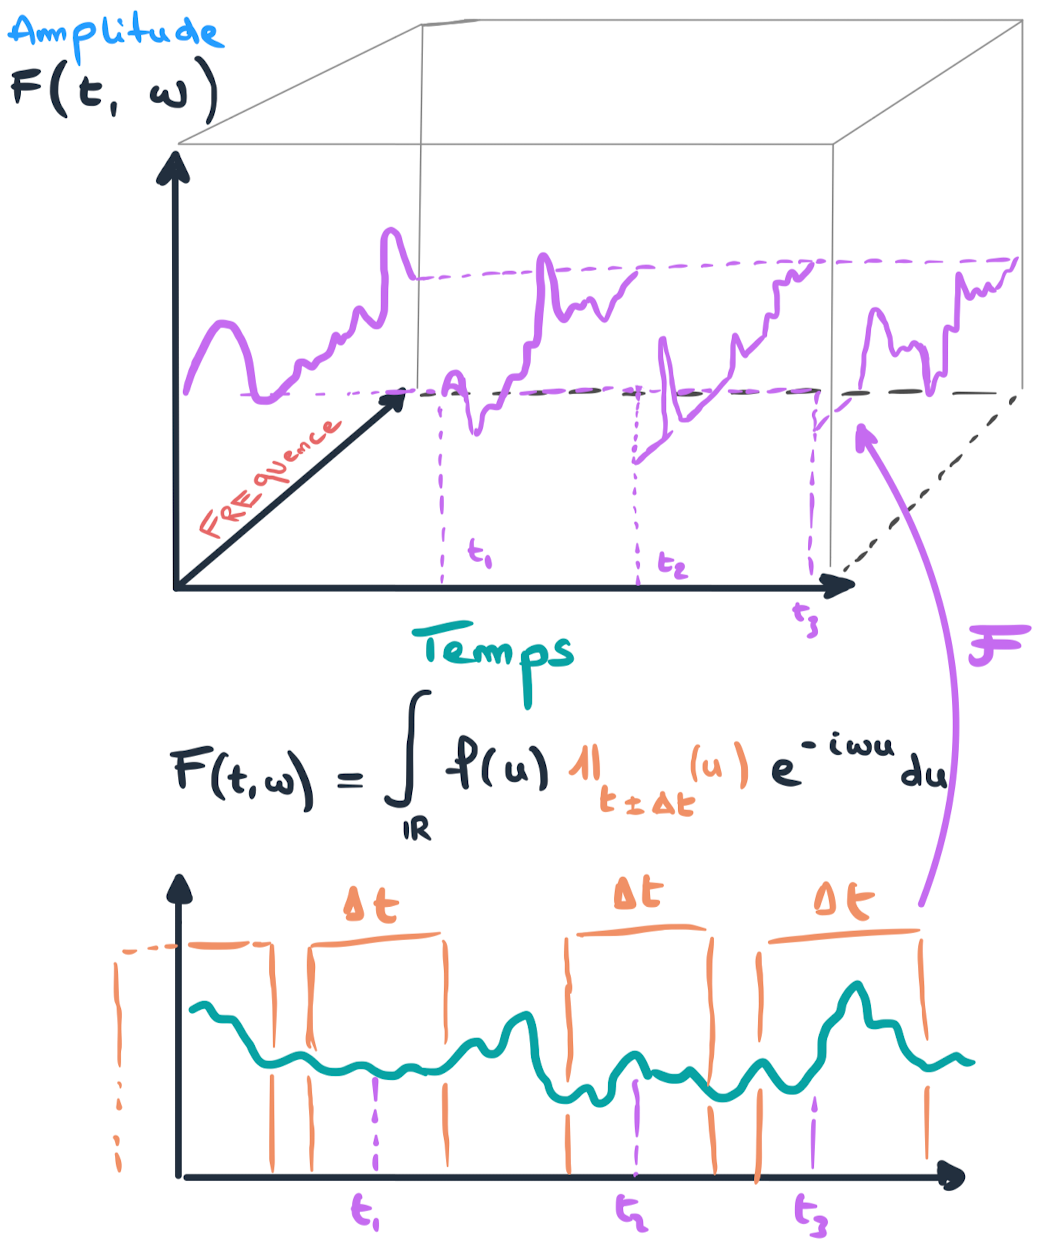
\includegraphics[width=\textwidth]{images/sketches/STFT.png}
        \caption{Transformée de Fourier à court terme d'une fonction}
        \label{fig:STFT}
    \end{figure}
\end{minipage}
\hfill
\begin{minipage}{0.60 \textwidth}
 
    Cependant contrairement à ce que peut suggérer le dessin présenté ici, la résolution fréquentielle n'est pas parfaite. Elle est d'ailleurs dans le cadre de la Transformée de Fourier à court terme constante, que ce soit sur le domaine temporel ou le domaine fréquentiel. La résolution fréquentielle est donc constante quelque soit la fréquence considérée.

    \question{
        \smallskip\centering
        Quel est le problème avec cette approche ?
    }

    le problème ne vient pas du monde mathématique mais plutôt du monde réel : les signaux que l'on observent présentent la caractéristique suivante : Les signaux de basse fréquence ont tendance à s'étendre sur la durée, et les signaux de hautes fréquences ont tendance à être très localisées, sous forme d'impulsion. Il devient alors clair que pour correctement identifier et localiser les fréquences présentes dans un signal, il est judicieux (voire parfois nécessaire) de varier la résolution fréquentielle et temporaire (limitées par le théorème d'indétermination de Heisenberg) en fonction de ce qui est le plus difficile à distinguer. C'est ce que proposent les ondelettes.
    
\end{minipage}

\subsubsection{Ondelettes}

\textbf{Transformée en ondelettes}

Introduisons maintenant de façon plus formelle les ondelettes et regardons leurs propriétés intéressantes dans le cadre du lissage de trajectoires.

on définit la transformée en ondelettes vis à vis de l'ondelette mère $\psi$ d'une fonction $f$ par :

$$F : \begin{array}{ccc}
  \mathds R \times \mathds R_+  &\longrightarrow & \mathds R
    \\
   (t,s) & \longmapsto & \displaystyle\frac 1 { \sqrt{|s|}} \int_{\mathds R} f(\colorize{u}) \psi \left( \frac{\colorize{u}-t}{s} \right) \mathrm d \colorize{u}
\end{array}$$

\brain{on peut remarquer que la formule de la transformée en ondelettes ressemble à une projection : $\displaystyle\frac{\langle f, \psi_{t,s} \rangle_{\mathds L^2}}{|| \psi_{t,s} ||}$. Cela vient en quelque sorte motiver la section suivante}

\textbf{Base d'ondelettes}

$$
\left( \psi_{k,n} : t \mapsto \frac 1 {\sqrt{2^k}} \psi( \frac{t - 2^k n}{2^k} ) \right)_{(k,n) \in \mathds Z^2} \textsf{ est une base } \underset {|| \cdot ||}{\perp} \textsf{ de } \mathds L^2
$$
 
\info{notons que les résolutions sont des puissances de 2, ceci est un détail qui demandera une implémentation particulière dans le cadre des données réelles : il faudra faire attention à ce que le nombre de points que l'on donne dans l'algorithme de transformée rapide en ondelettes soit aussi une puissance de 2.}

\textbf{Propriétés principales des ondelettes}

\smallskip

\begin{itemize}
    \item \textbf{Approximation dans l'espace fréquentiel-temporel} : La transofrmée en ondelettes ( $\mathcal W : f \mapsto \langle f \, | \, \psi_{t,s} \rangle$ ) est une isométrie de $\mathds L^2$. Cela nous permet donc d'affirmer que $|| f - \hat f ||_{\mathds L^2} = || \mathcal W f - \mathcal W \hat f ||_{\mathds L^2}$. Ainsi on peut travailler dans l'espace des ondelettes pour approximer (dans notre cas lisser les trajectoires) des fonctions et contrôler l'approximation directement dans le domaine fréquence-temporel tout en le conservant dans le domaine temporel. \citationrequise
    % @ todo : compléter citation — STFT : talk de Stéphane Mallat

    \item \textbf{Propriété de Fast Decay}
\end{itemize}





\subsubsection{Motivation dans le cadre de l'analyse de données fonctionnelles}

\subsubsection{Effets du lissage à ondelettes sur la régularité locale}

\section{Estimation adaptative}

\subsection{Estimation adaptative de la fonction moyenne}

\subsection{Estimation adaptative de l'opérateur de covariance}

\subsection{Estimation adaptative de l'auto-covariance des séries temporelles fonctionnelles}